\documentclass[a4paper,14pt]{extreport} % формат документа

\usepackage{amsmath}
\usepackage{cmap} % поиск в ПДФ
\usepackage[T2A]{fontenc} % кодировка
\usepackage[utf8]{inputenc} % кодировка исходного текста
\usepackage[english,russian]{babel} % локализация и переносы
\usepackage[left = 2cm, right = 1cm, top = 2cm, bottom = 2 cm]{geometry} % поля
\usepackage{listings}
\usepackage{graphicx} % для вставки рисунков
\usepackage{amsmath}
\usepackage{float}
\usepackage{multirow}
\graphicspath{{img/}}
\DeclareGraphicsExtensions{.pdf,.png,.jpg}
\newcommand{\anonsection}[1]{\section*{#1}\addcontentsline{toc}{section}{#1}}

\lstset{ %
	language=Lisp,                % Язык программирования 
	numbers=left,                   % С какой стороны нумеровать          
	frame=single,                    % Добавить рамку
}

\begin{document}
\begin{titlepage}

    \begin{table}[H]
        \centering
        \footnotesize
        \begin{tabular}{cc}
            \multirow{8}{*}{
\includegraphics[scale=0.35]{bmstu.jpg}}
            & \\
            & \\
            & \textbf{Министерство науки и высшего образования Российской Федерации} \\
            & \textbf{Федеральное государственное бюджетное образовательное учреждение} \\
            & \textbf{высшего образования} \\
            & \textbf{<<Московский государственный технический} \\
            & \textbf{университет имени Н.Э. Баумана>>} \\
            & \textbf{(МГТУ им. Н.Э. Баумана)} \\
        \end{tabular}
    \end{table}

    \vspace{-2.5cm}

    \begin{flushleft}
        \rule[-1cm]{\textwidth}{3pt}
        \rule{\textwidth}{1pt}
    \end{flushleft}

    \begin{flushleft}
        \small
        ФАКУЛЬТЕТ
        \underline{<<Информатика и системы управления>>\ \ \ \ \ \ \ 
        \ \ \ \ \ \ \ \ \ \ \ \ \ \ \ \ \ \ \ \ \ \ \ \ \ \ \ \ \ \ \ 
    \ \ \ \ \ \ \ \ \ \ \ \ \ \ \ } \\
        КАФЕДРА
        \underline{<<Программное обеспечение ЭВМ и
        информационные технологии>>
        \ \ \ \ \ \ \ \ \ \ \ \ \ \ \ \ \ \ \ \ }
    \end{flushleft}

    \vspace{2cm}

    \begin{center}
        \textbf{Лабораторная работа № 2} \\
        \vspace{0.5cm}
    \end{center}

    \vspace{4cm}

    \begin{flushleft}
        \begin{tabular}{ll}
            \textbf{Дисциплина} & Экономика программной инженерии.  \\
            \textbf{Тема} & Определение ресурсов и затрат для проекта \\
            \\
            \textbf{Студент} & Сиденко А.Г. \\
            \textbf{Группа} & ИУ7-83Б \\
            \textbf{Оценка (баллы)} & \\
            \textbf{Преподаватель} & Барышникова М.Ю., Силантьева А.В.   \\
        \end{tabular}
    \end{flushleft}

    \vspace{4cm}

   \begin{center}
        Москва, 2021 г.
    \end{center}

\end{titlepage}

\begin{enumerate}
\item \textbf{Тренировочное задание}

Заполняем ресурсный лист исполнителями и материальным ресурсом.

\begin{figure}[H]
  \centering
  \caption{Ресурсы. }
  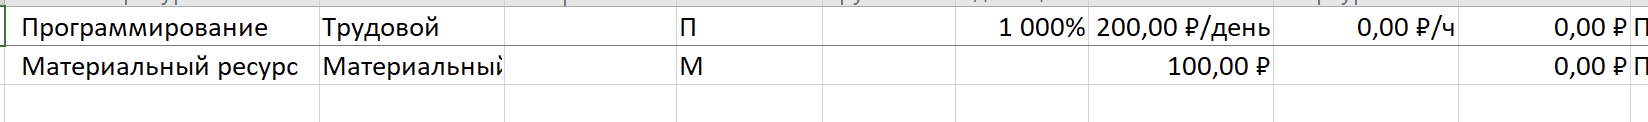
\includegraphics[scale=0.6]{dop}
\end{figure}

Далее назначаем ресурсы на задачи.

\begin{figure}[H]
  \centering
  \caption{Задачи. }
  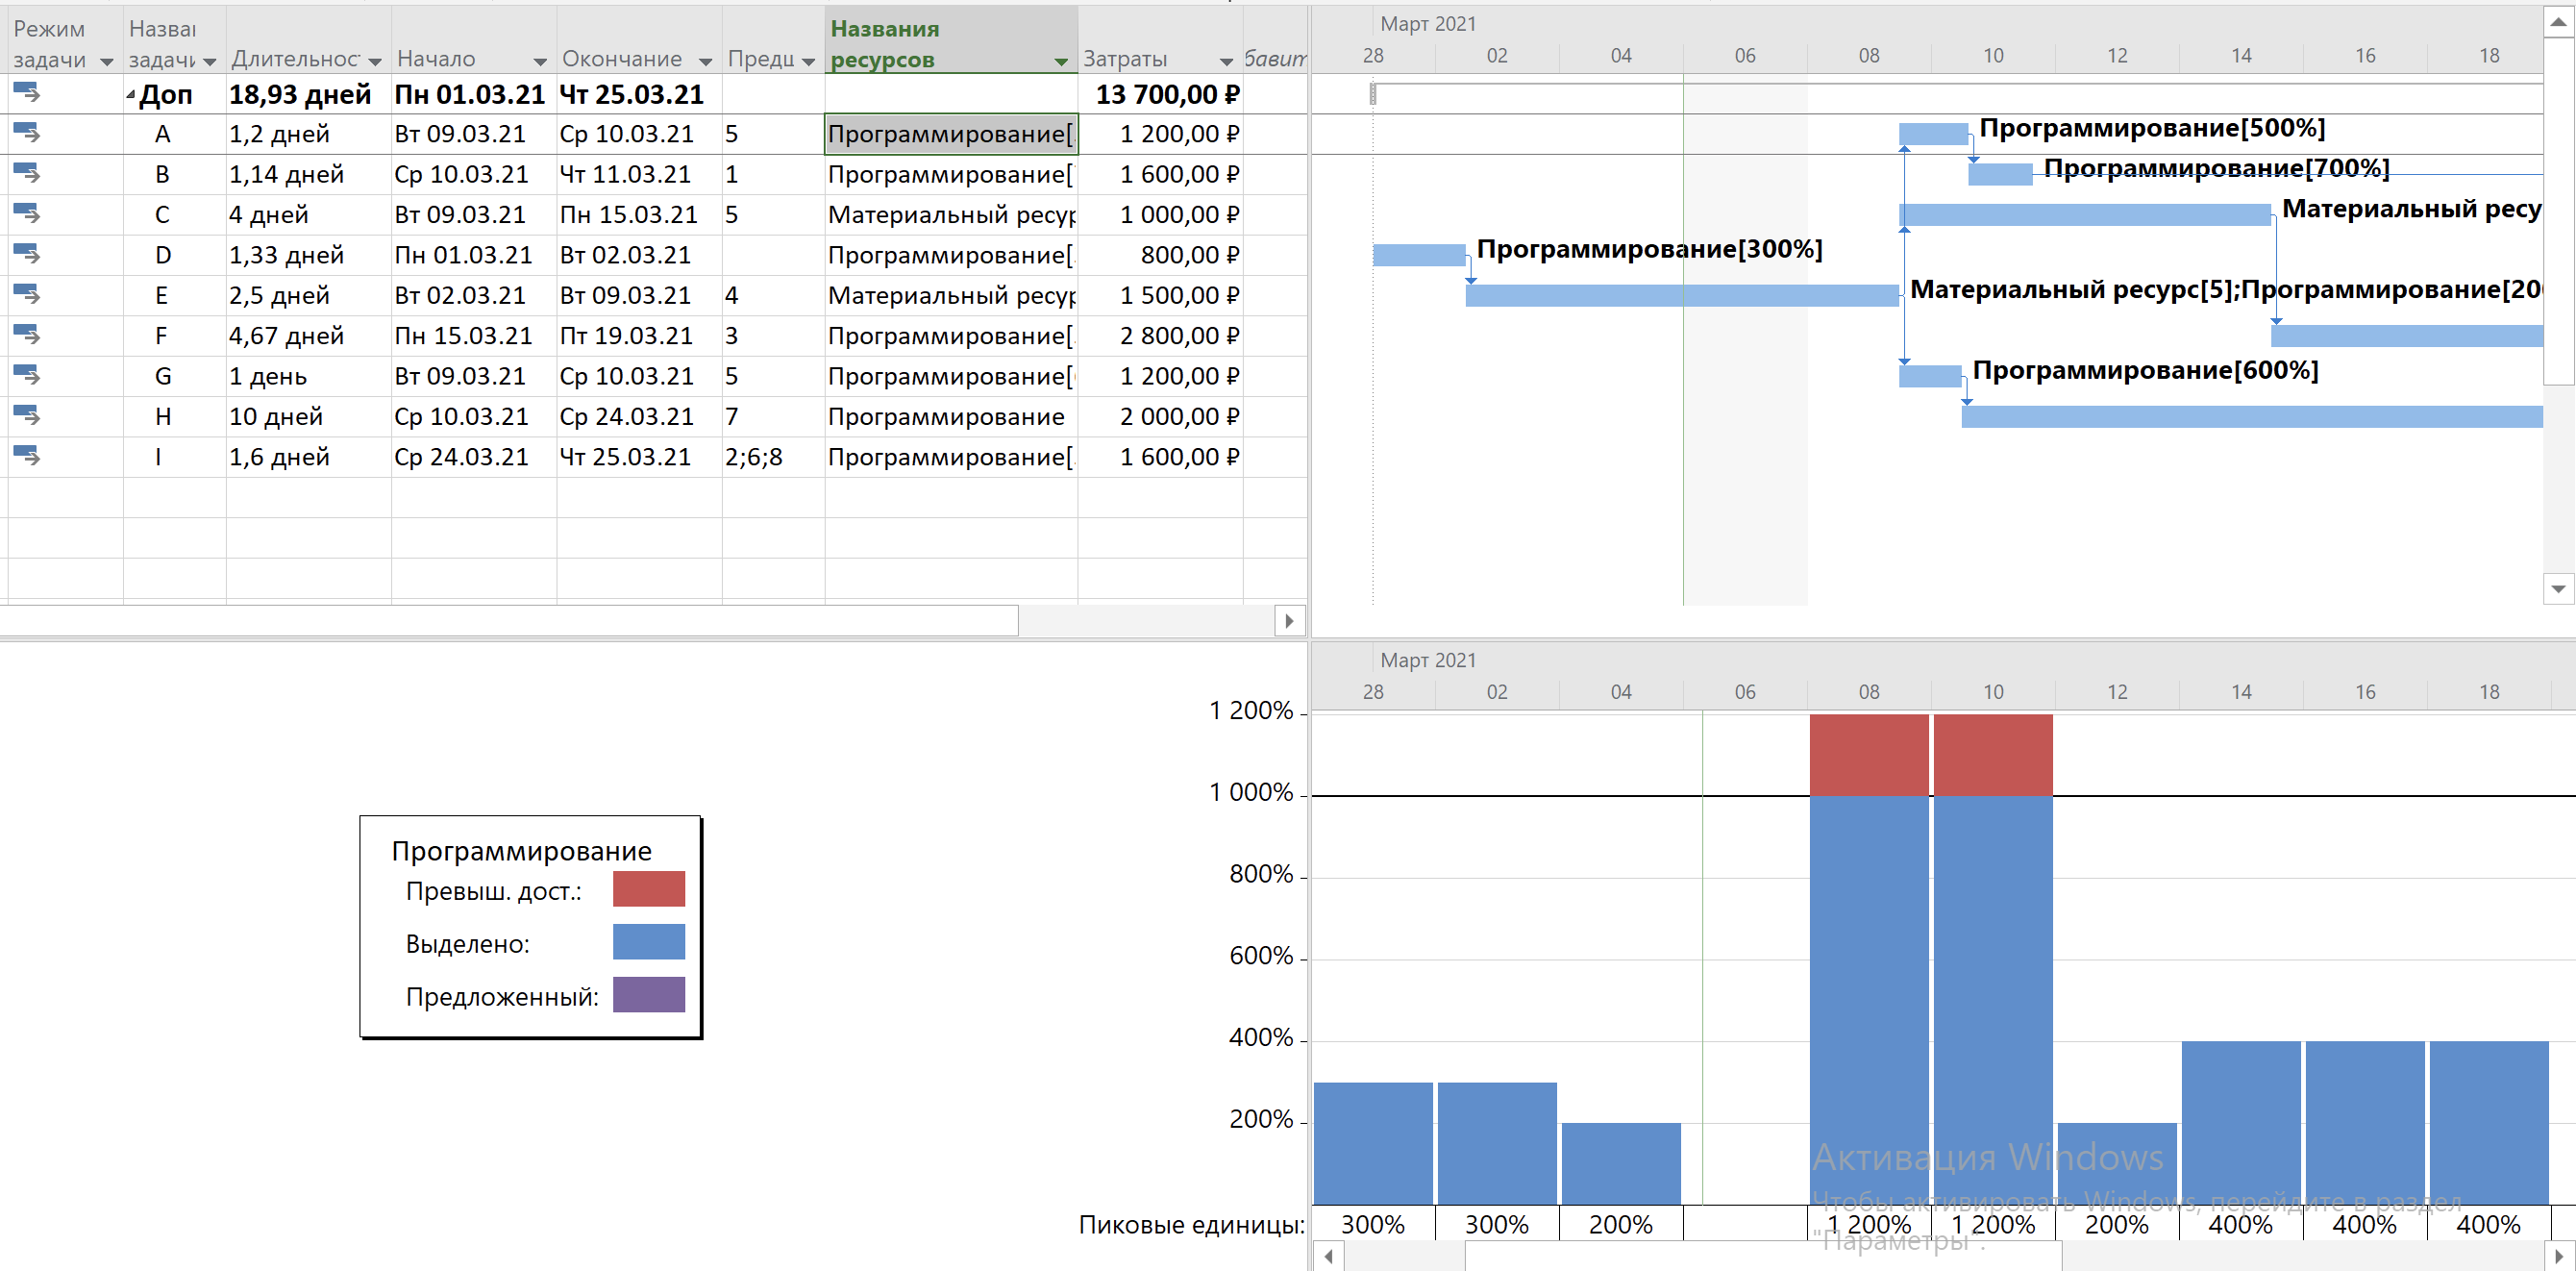
\includegraphics[scale=0.38]{dop1}
\end{figure}

Ресурсы перегружены на 200\%.

\item \textbf{Основное задание}

Содержание проекта: Команда разработчиков из 16 человек занимается созданием карты города на основе собственного модуля отображения. Проект должен быть завершен в течение 6 месяцев. Бюджет проекта: 50 000 рублей.

\item \textbf{Задание 1}

Заполняем ресурсный лист.

\begin{figure}[H]
  \centering
  \caption{Ресурсный лист. }
  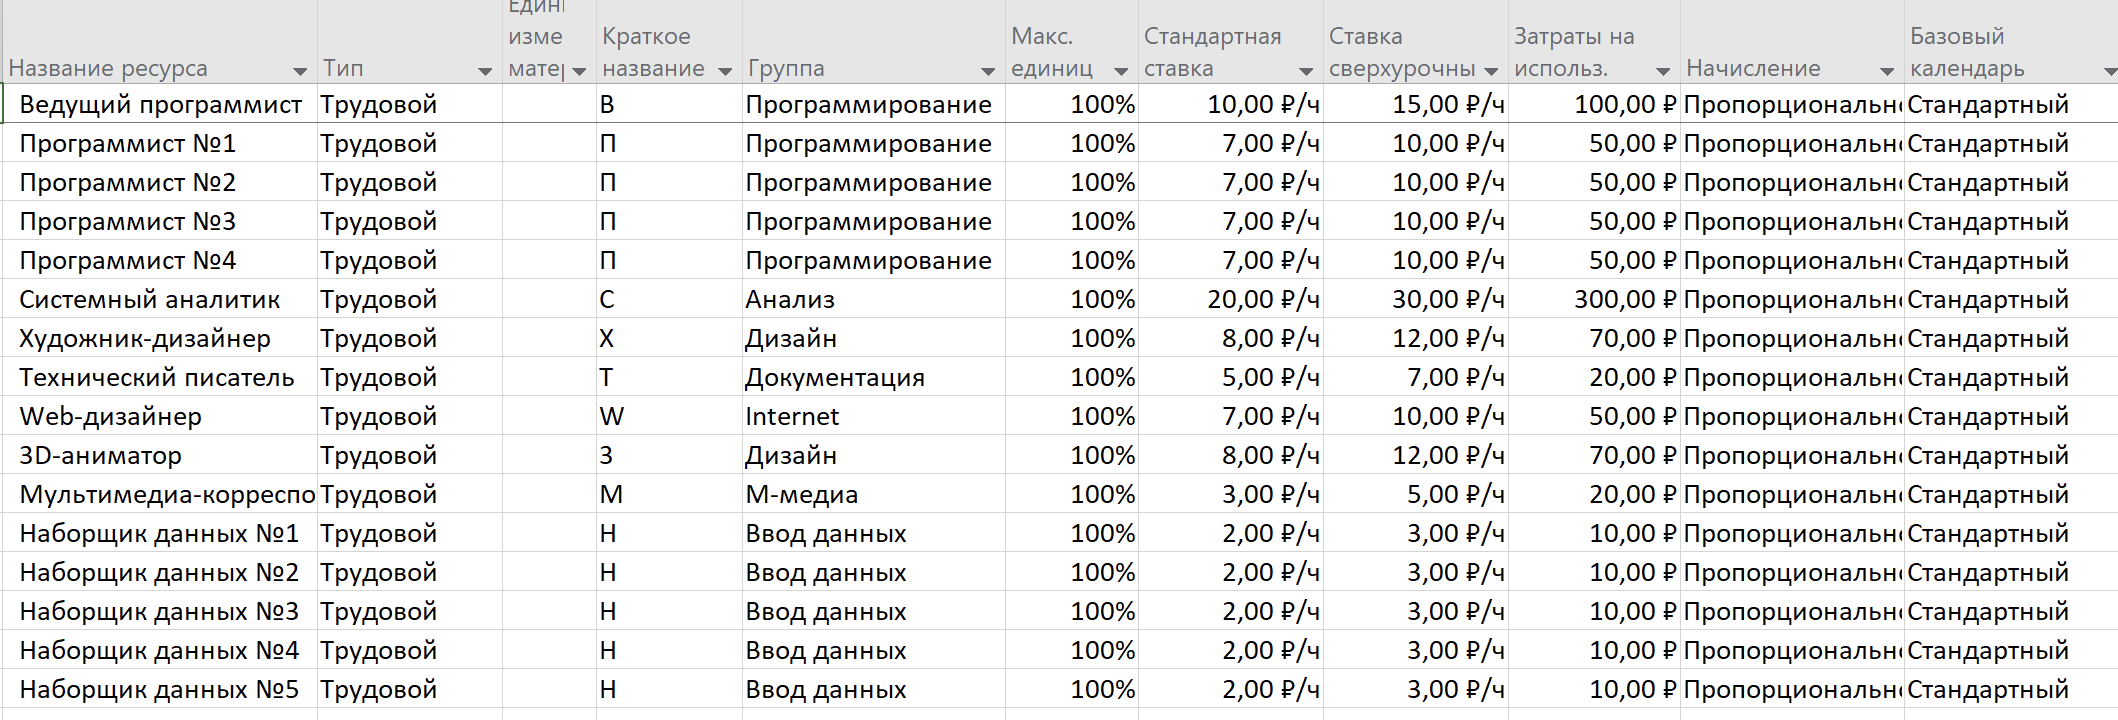
\includegraphics[scale=0.5]{list}
\end{figure}

\item \textbf{Задание 2}

Назначаем ресурсам задачи. Дополнительно для задачи 8 арендуем сервер (он работает 24 часа в сутки). 

\begin{figure}[H]
  \centering
  \caption{Список задач. }
  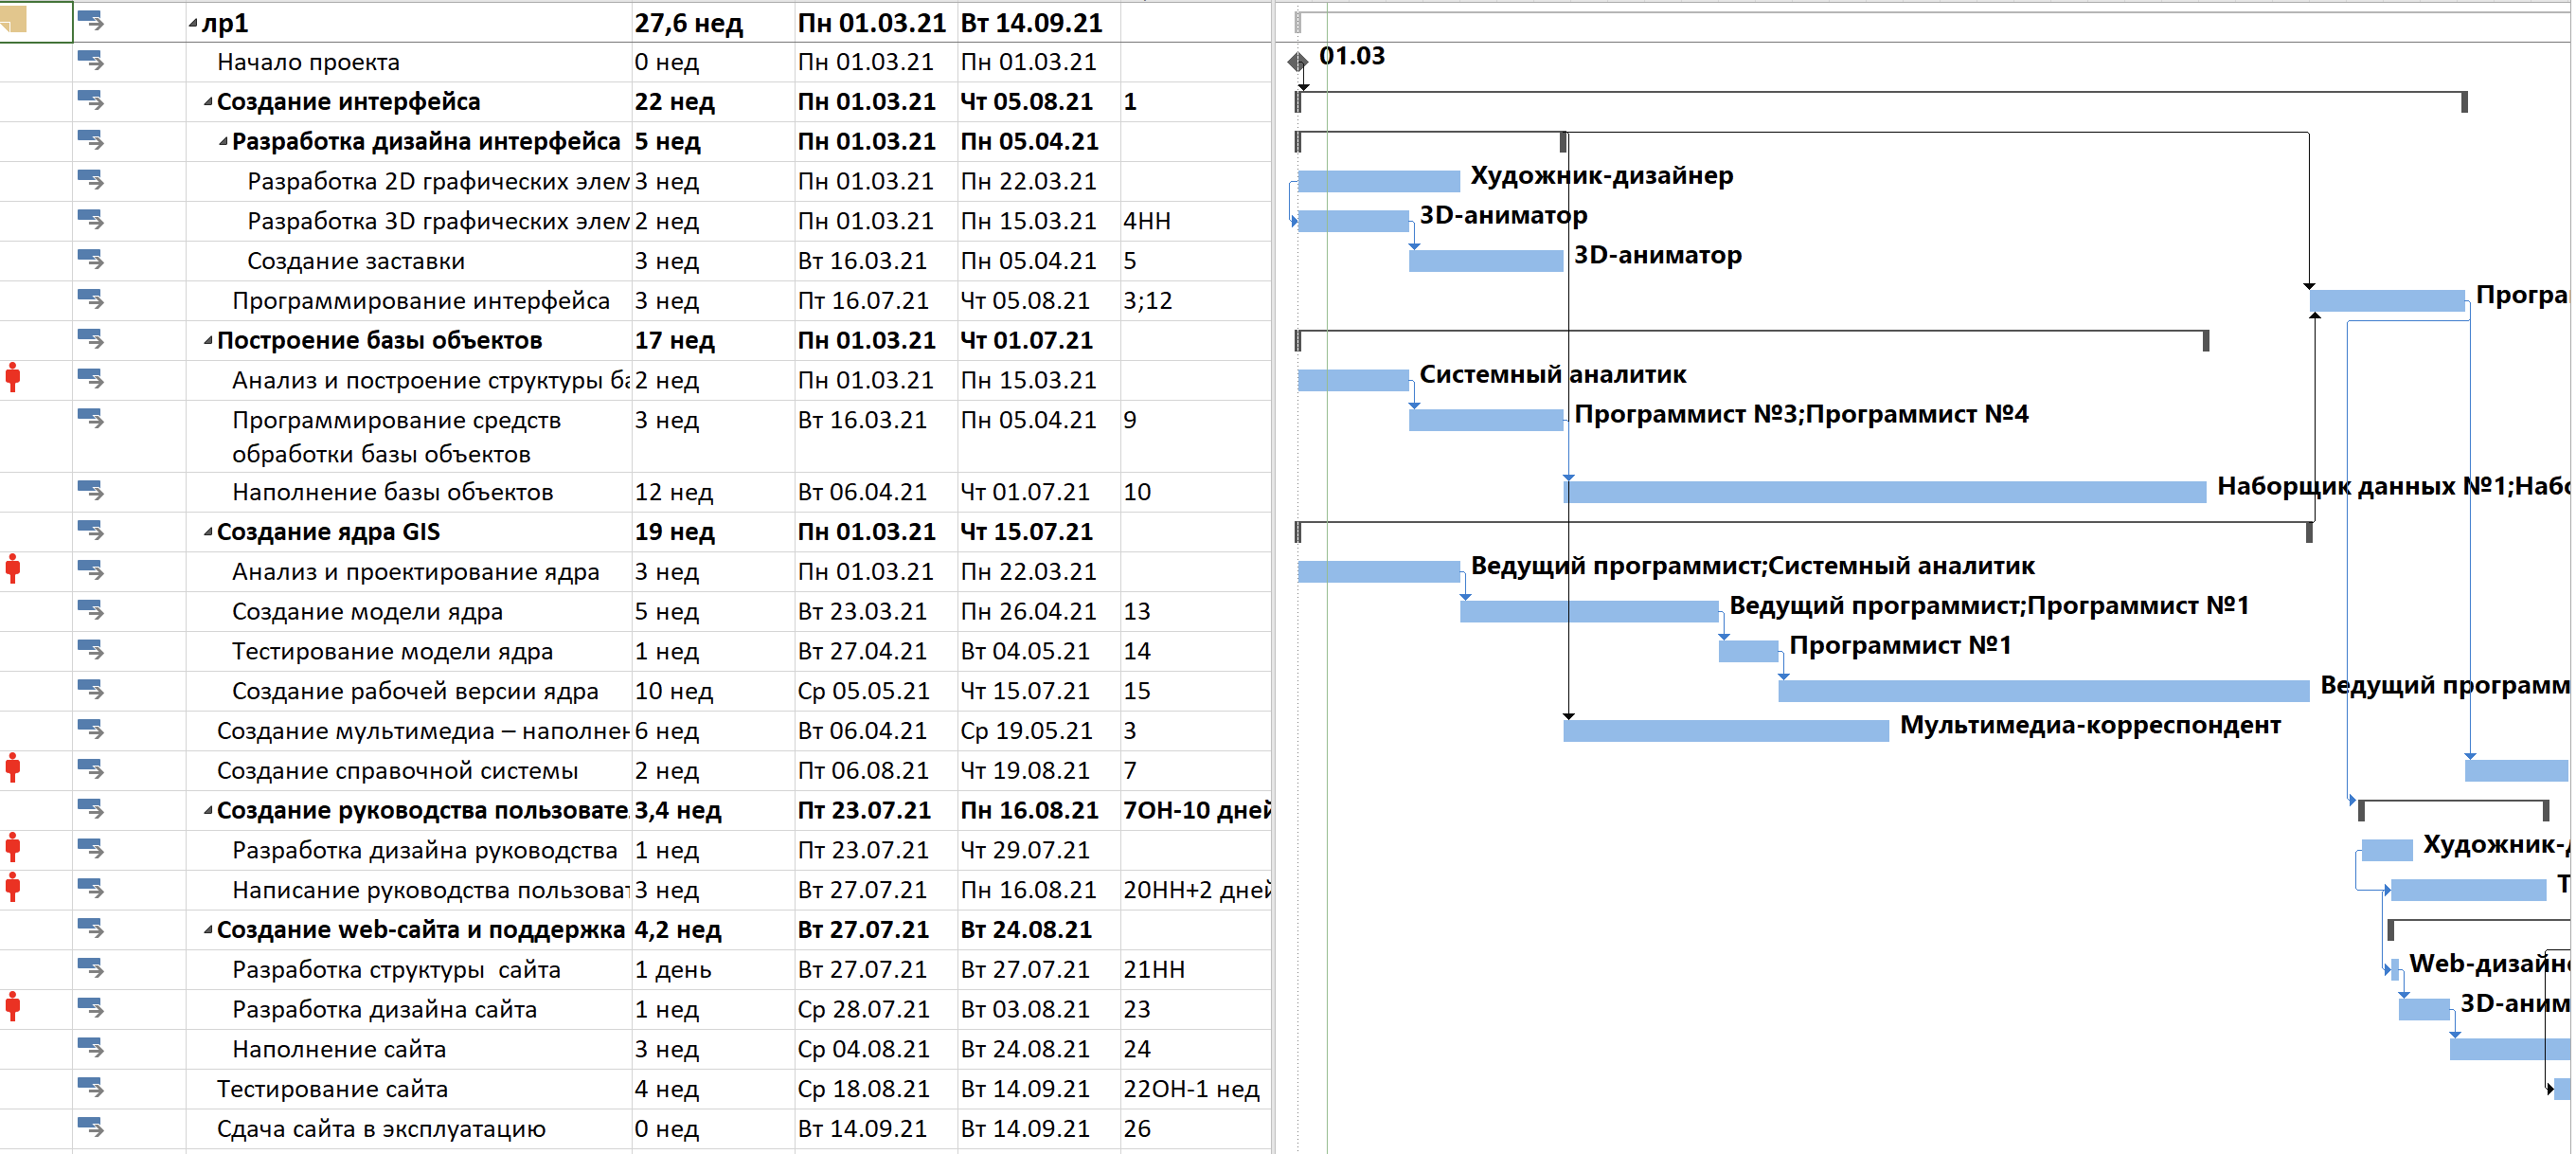
\includegraphics[scale=0.39]{2}
\end{figure}

Перегрузка ресурсов:
\begin{enumerate}
\item Системный аналитик -- одновременно выполняет задачи 9 (Анализ и построение структуры базы объектов ) и 13 (Анализ и проектирование ядра ).
\item Технический писатель -- одновременно выполняет задачи 21 (Написание руководства пользователя) и 18 (Создание справочной системы).
\item Художник-дизайнер -- одновременно выполняет задачи 20 (Разработка дизайна руководства) и 24 (Разработка дизайна сайта).
\end{enumerate}

\begin{figure}[H]
  \centering
  \caption{Использование сервера. }
  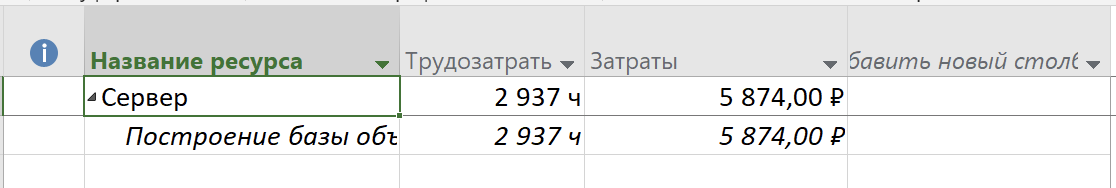
\includegraphics[scale=0.7]{server}
\end{figure}

Добавим фиксированные затраты для задач 2, 8 и 12.

\begin{figure}[H]
  \centering
  \caption{Затраты. }
  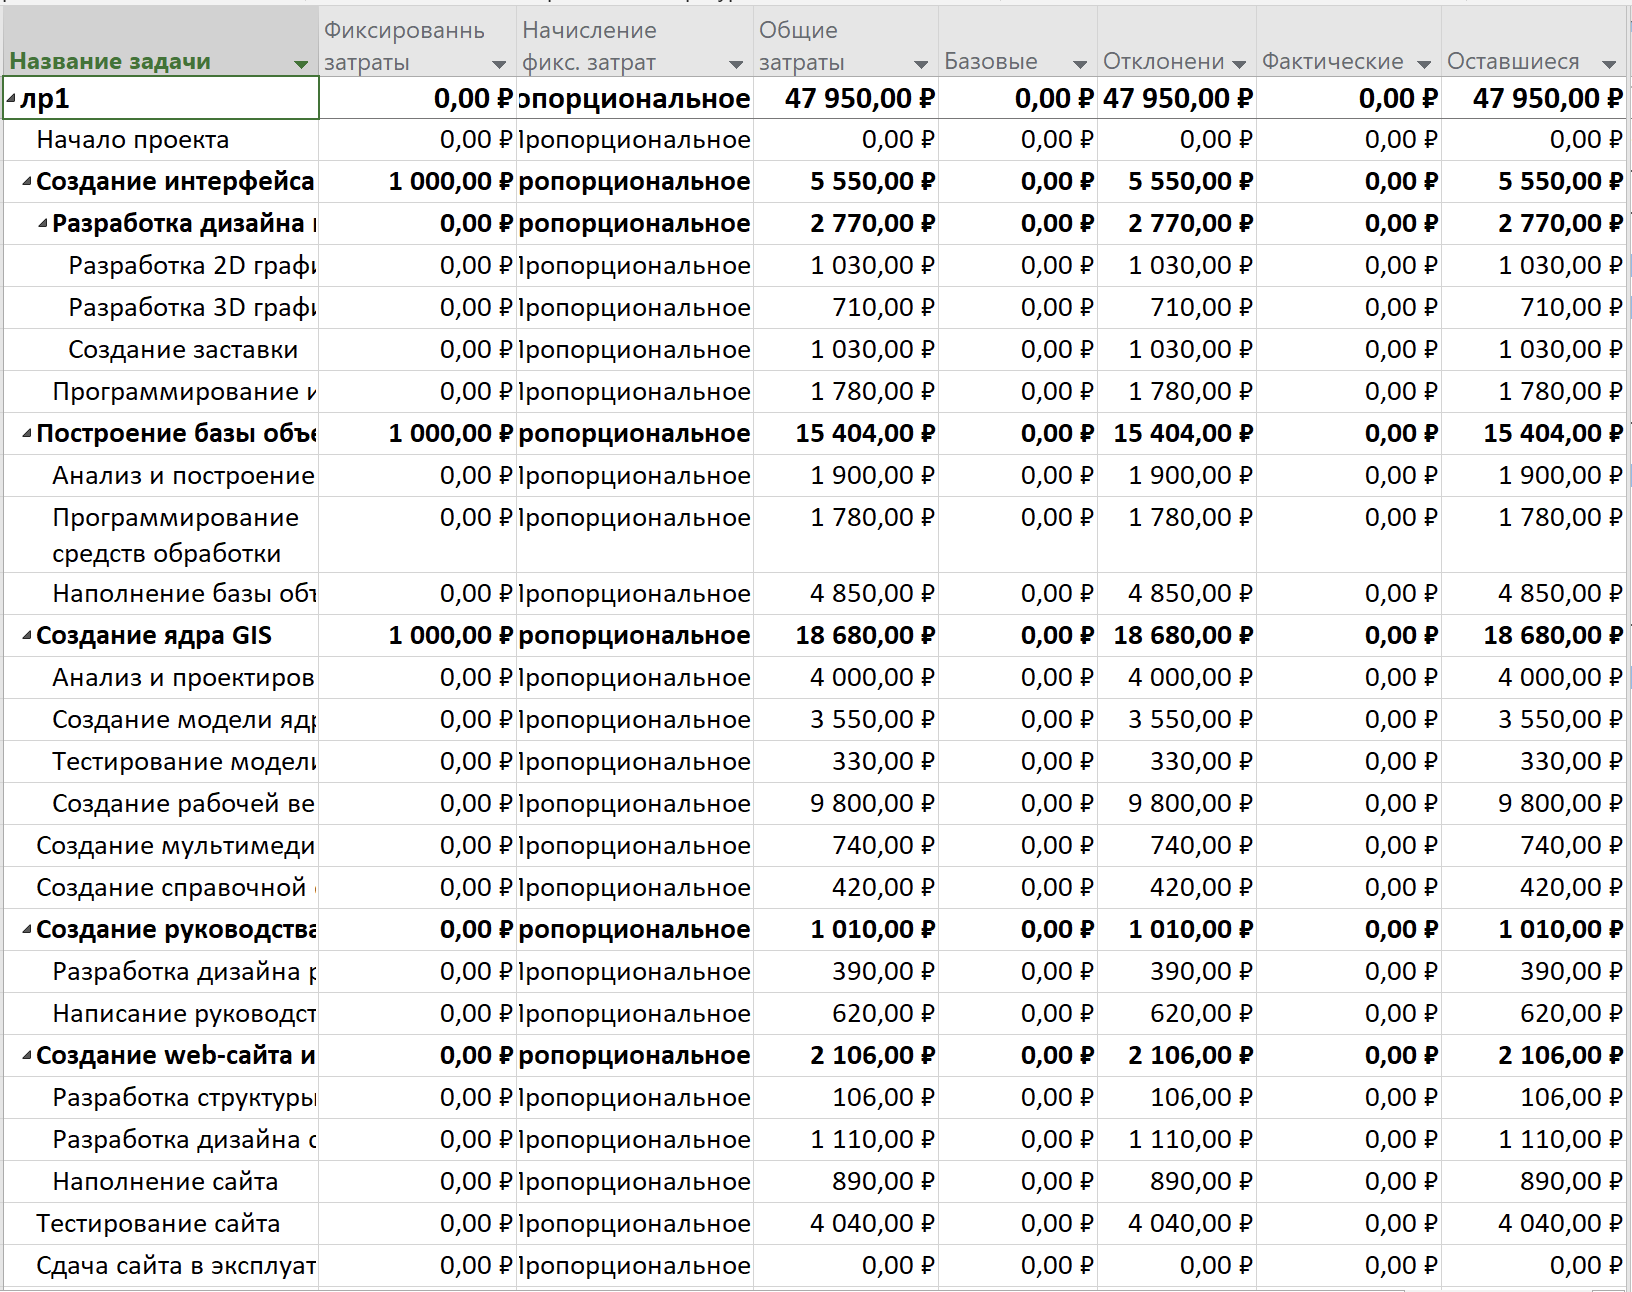
\includegraphics[scale=0.6]{expenses}
\end{figure}

\item \textbf{Задание 3}

Анализ затрат по группам ресурсов.

Заходим в представление Использование ресурсов и устанавливаем группировку.

\begin{figure}[H]
  \centering
  \caption{Затраты по группам ресурсов. }
  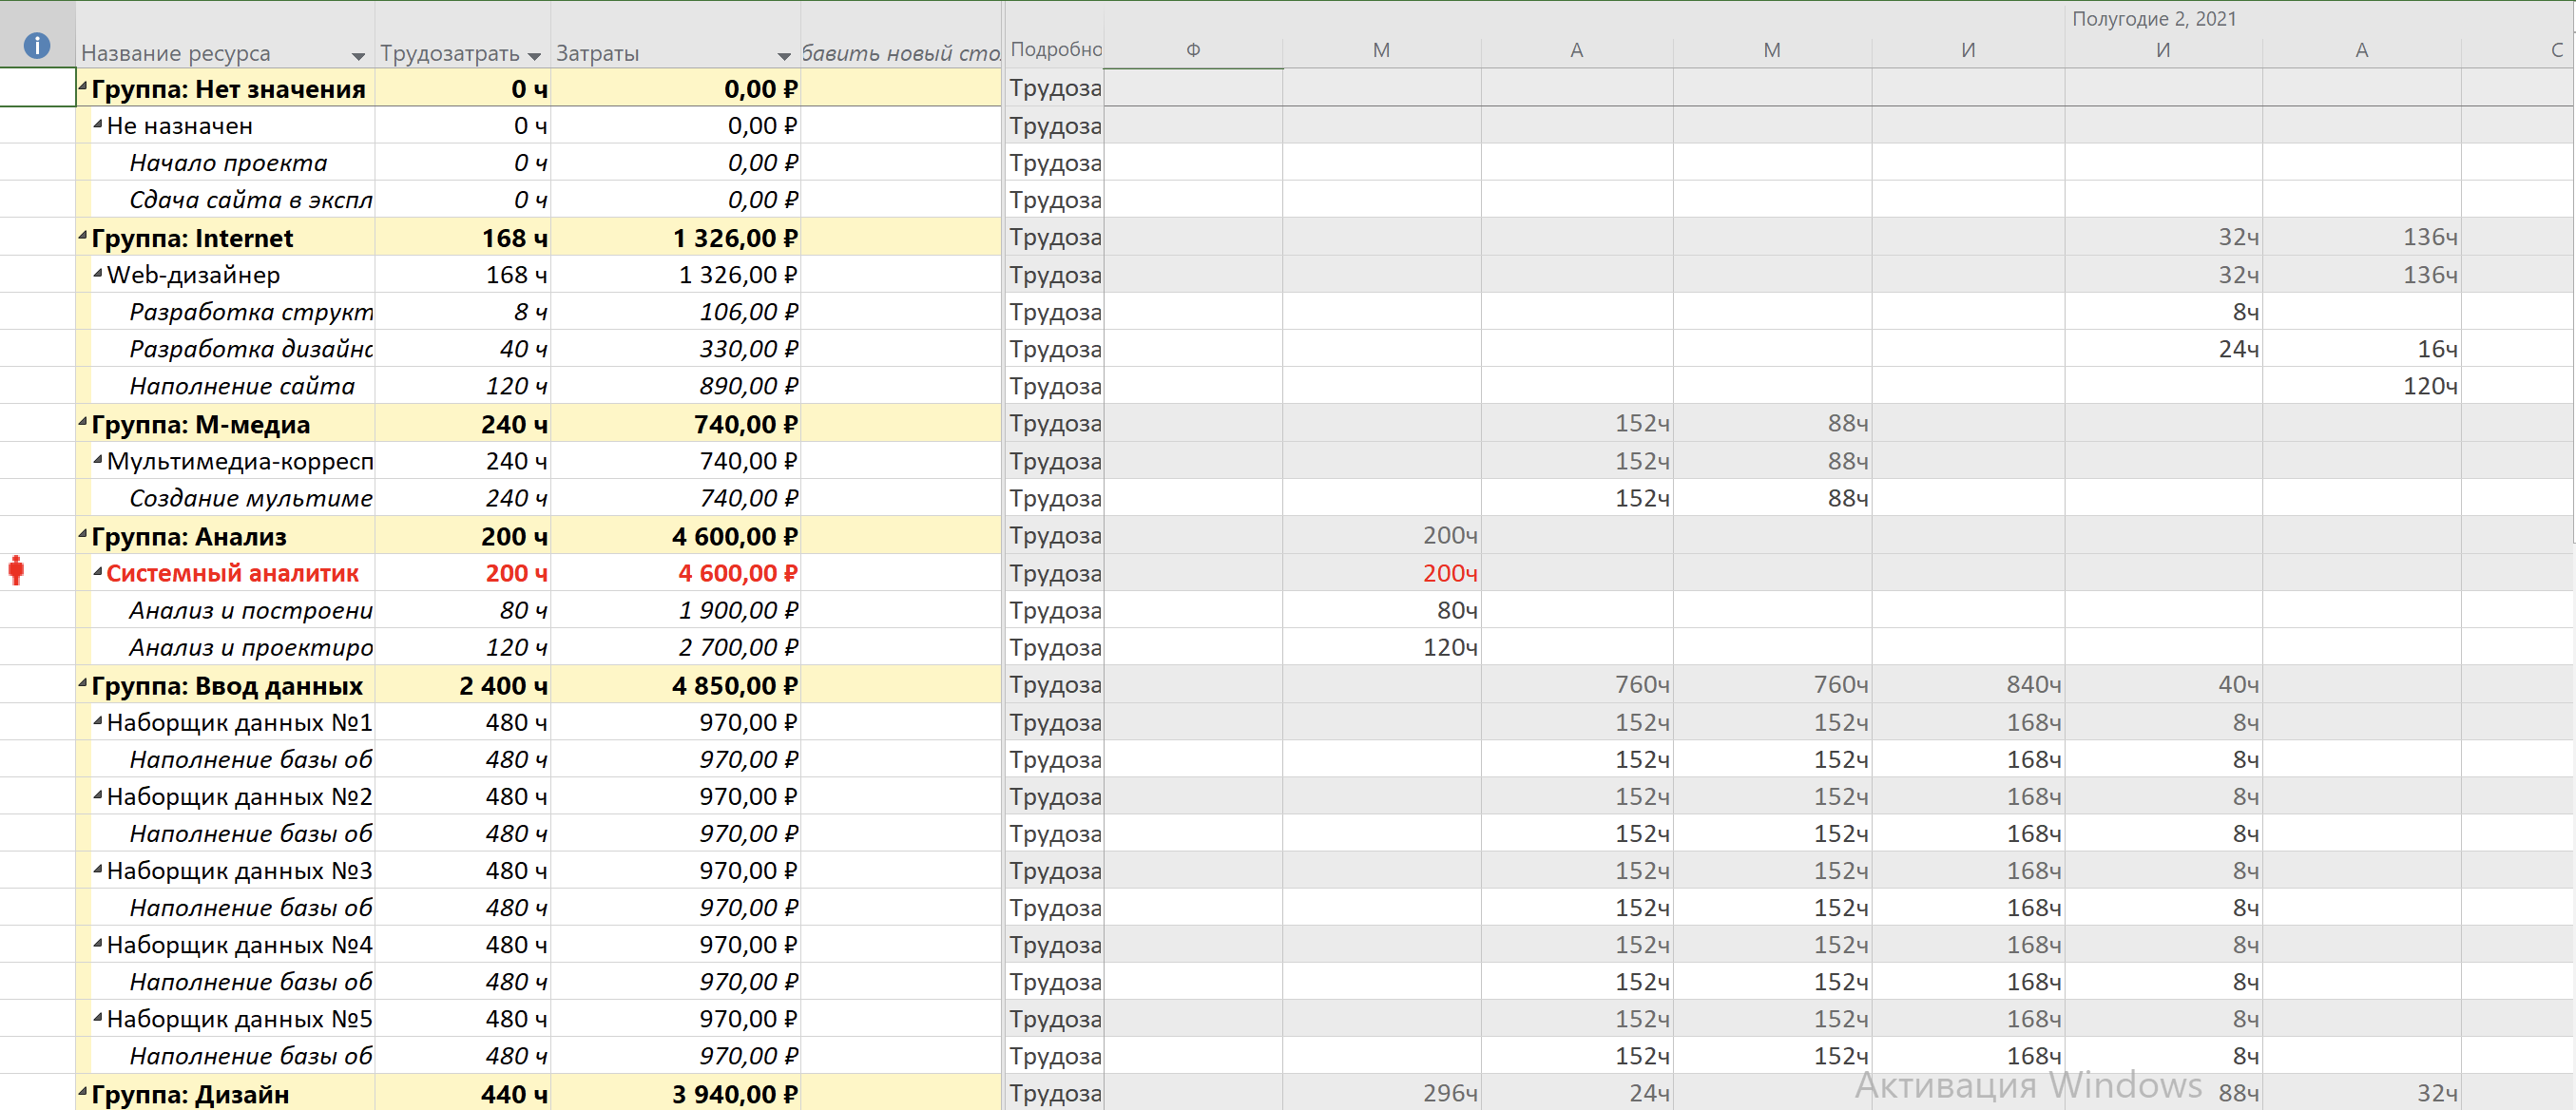
\includegraphics[scale=0.39]{3}
  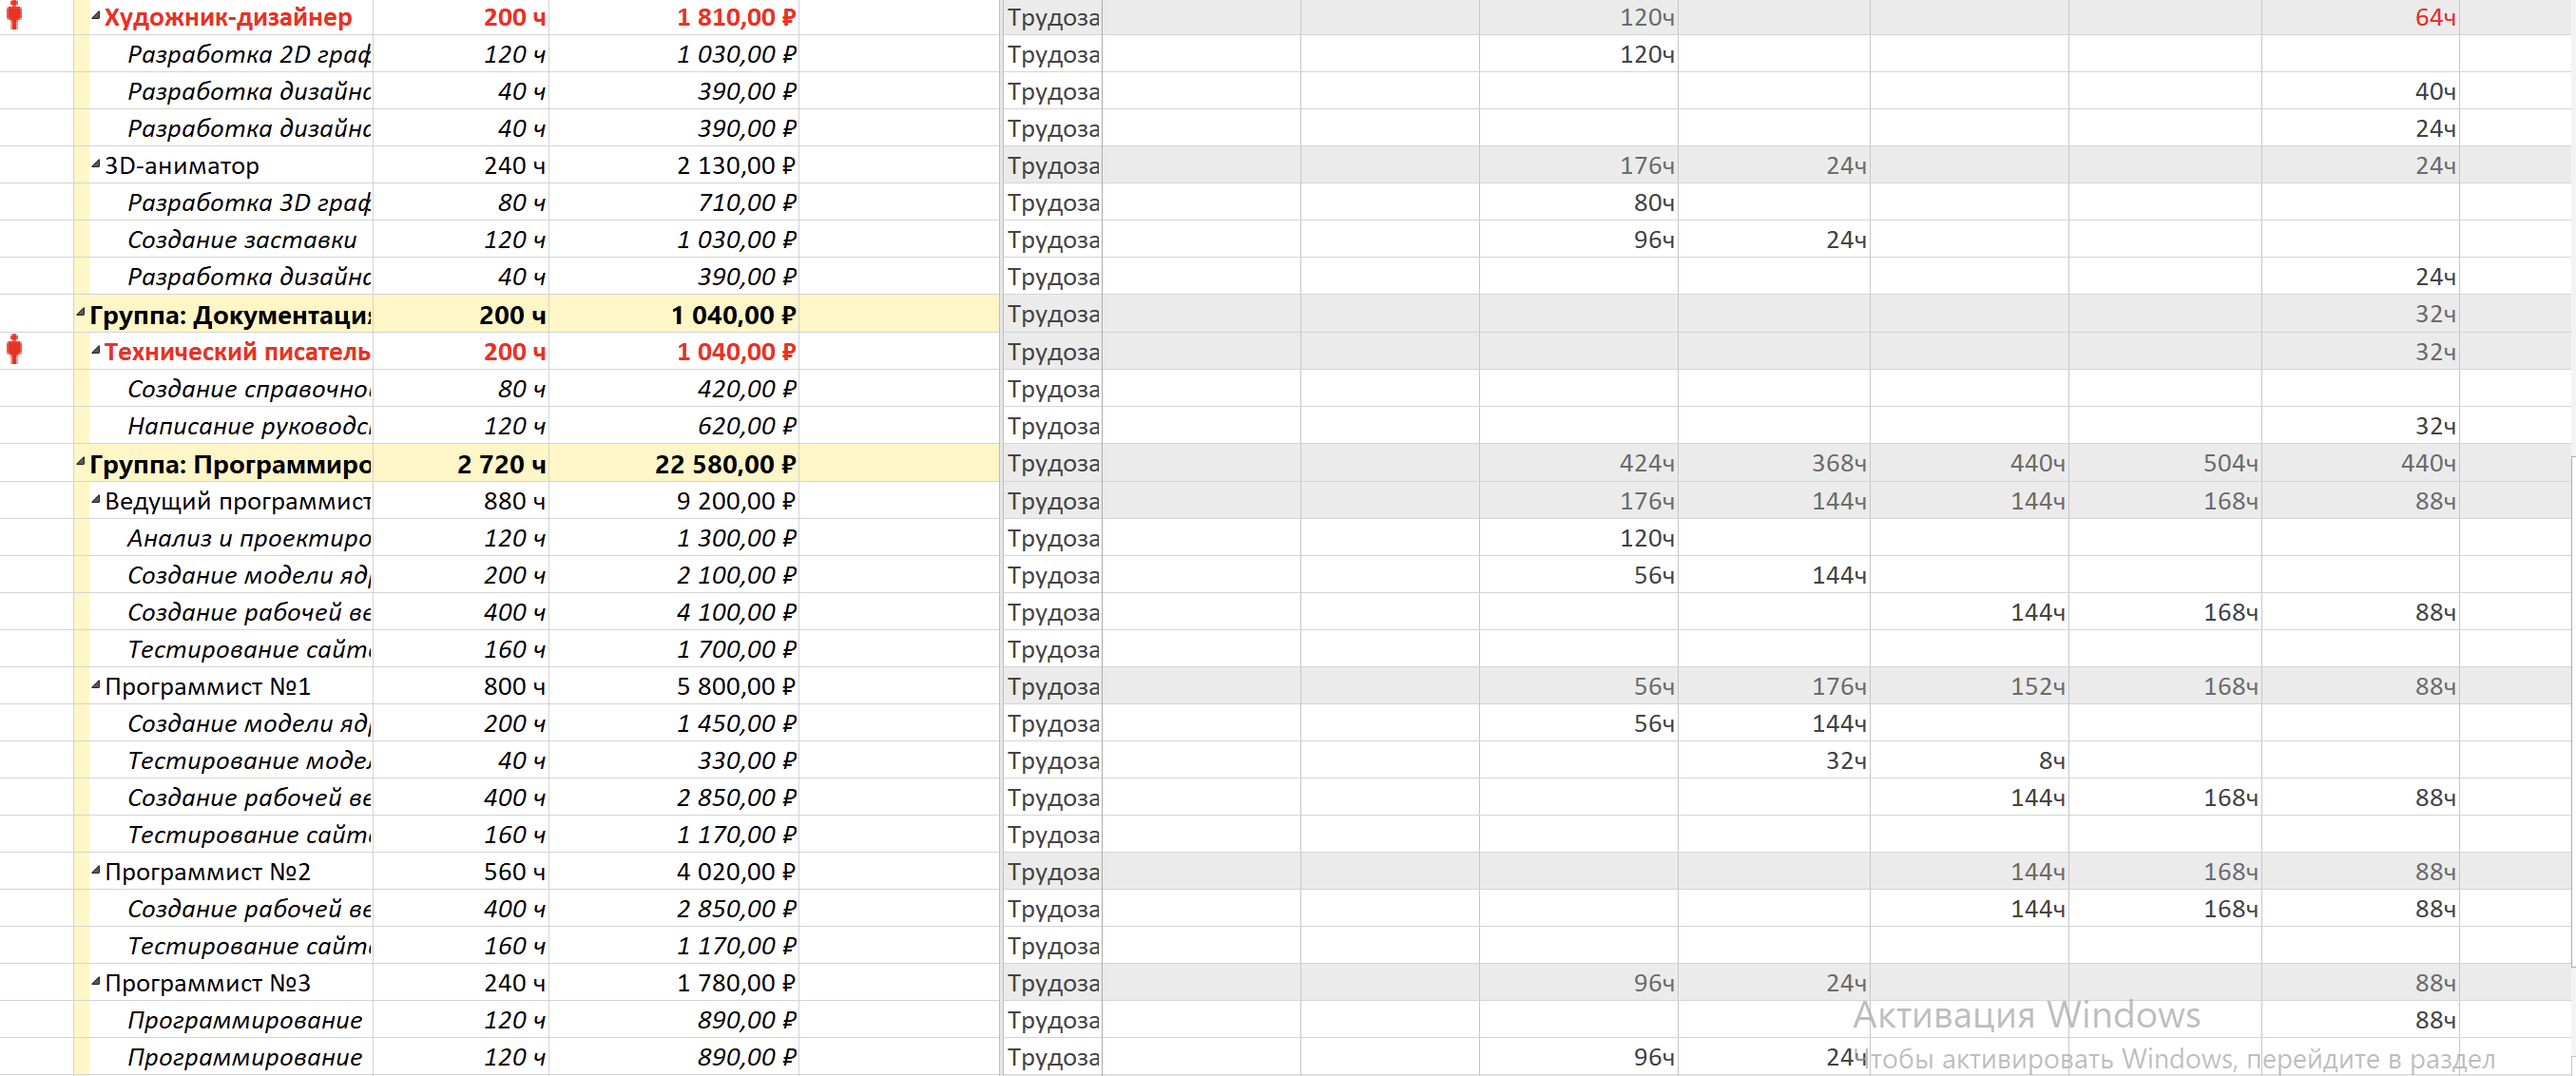
\includegraphics[scale=0.39]{4}
  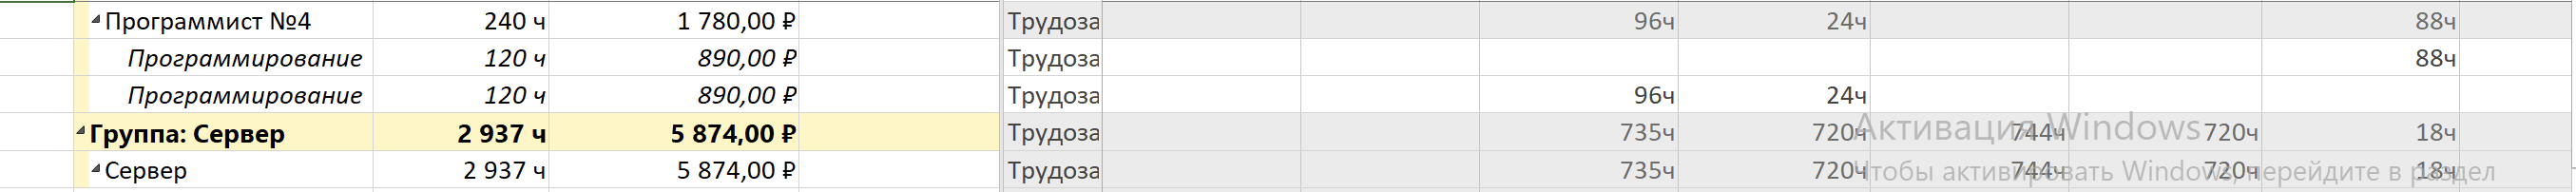
\includegraphics[scale=0.39]{5}
\end{figure}

Для графического представления воспользуемся MS Excel.

\begin{figure}[H]
  \centering
  \caption{Таблица. }
  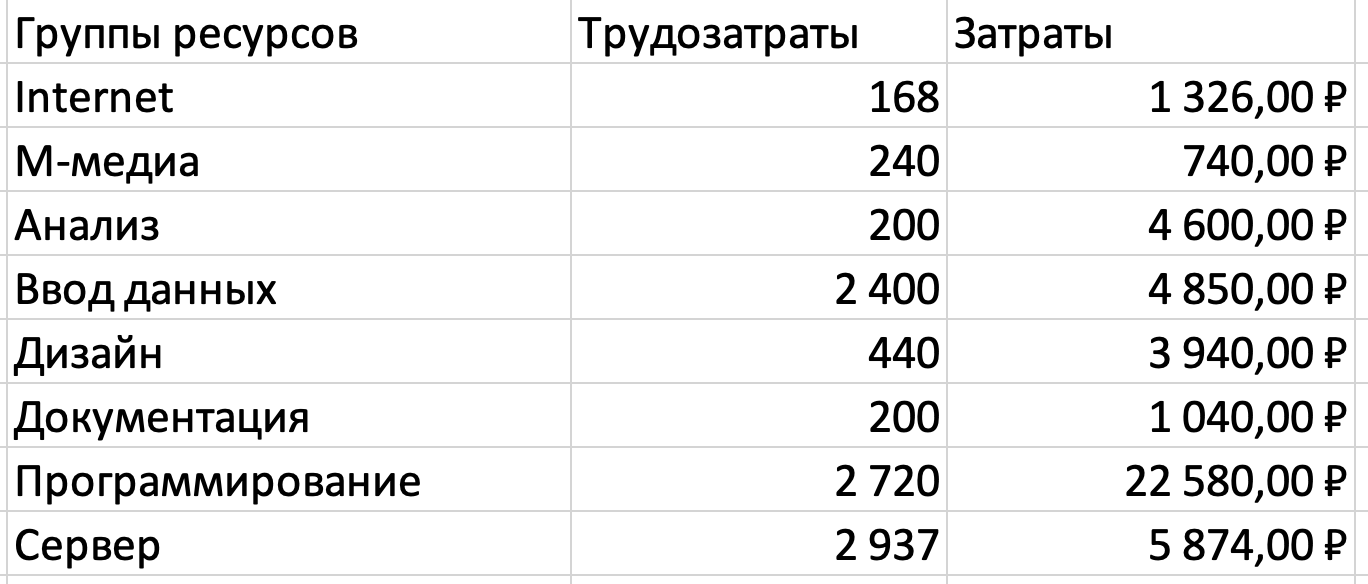
\includegraphics[scale=0.5]{table}
\end{figure}

\begin{figure}[H]
  \centering
  \caption{Информация о затратах по структурным группам ресурсов. }
  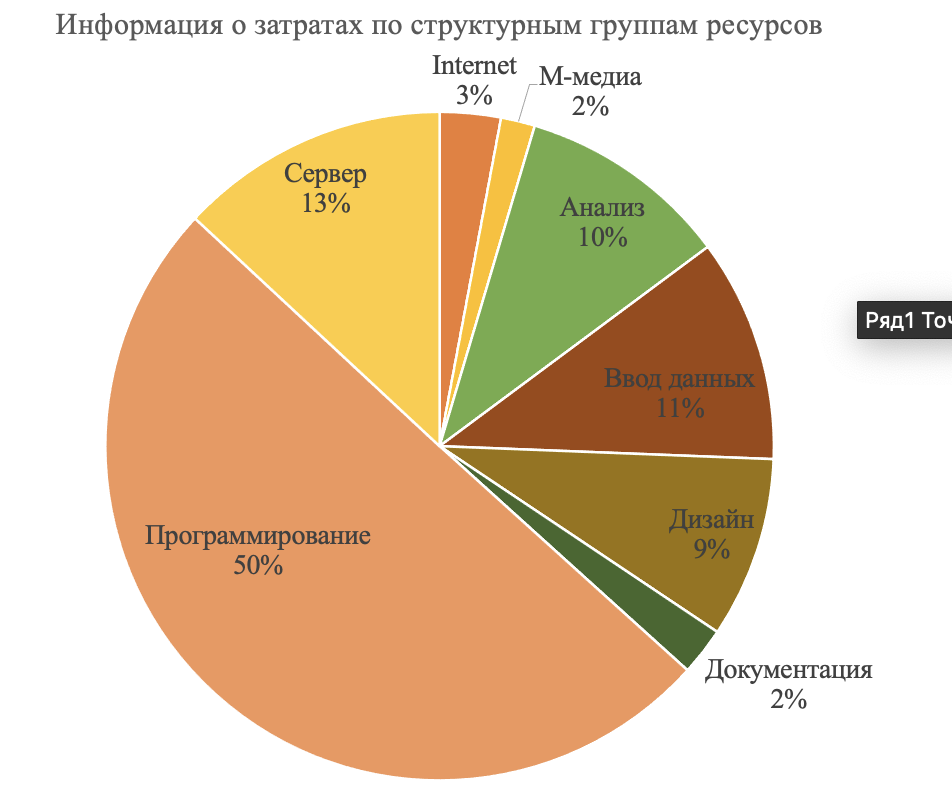
\includegraphics[scale=0.75]{d1}
\end{figure}

\begin{figure}[H]
  \centering
  \caption{Информация о трудозатратах по структурным группам ресурсов. }
  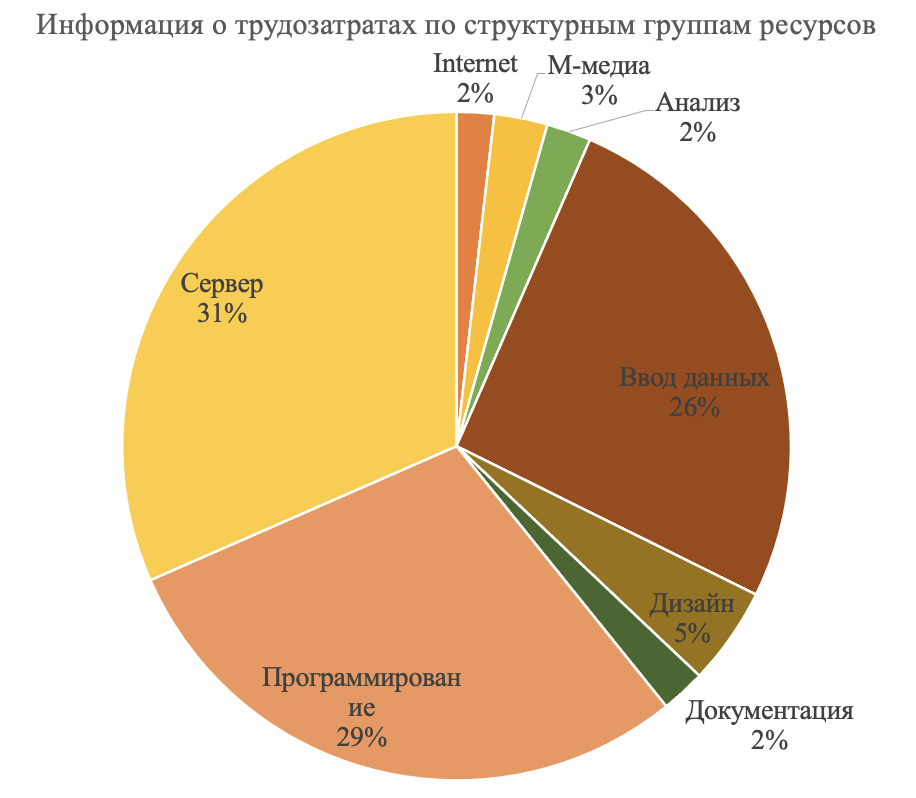
\includegraphics[scale=0.75]{d2}
\end{figure}

Как видим, на программистов приходится большая часть и затрат 50\%, и трудозатрат 29\%.

На сервер приходится 13\% затрат.

Также одной из больших затрат является аналитик 10\%, хотя выполняет всего 2\%.

Также затраты на ввод данных (наборщиков текста) составляют 11\% от общего бюджета, несмотря на то, что они выполняют 26\% работы.

Во всех остальных случаях объем работ и деньги в процентном соотношении примерно эквивалентны.

\item \textbf{Вывод}

В ходе выполнения лабораторной работы No2 продолжается изучение основных возможностей Microsoft Project 2019. Были созданы списки ресурсов, назначены ресурсы задачам и проведен анализ затрат по группам ресурсов.

В результате было выяснено, что программный проект укладывается в выделенный бюджет (47 950 рублей из 50 000 рублей). Но остается совсем небольшой запас денег, также системный аналитик, художник-дизайнер и технический писатель перегружены.

\end{enumerate}

\end{document}